	
\documentclass[thmsb,11pt]{article}
\usepackage{amsfonts}
\usepackage{appendix}
\usepackage[pagewise,displaymath, mathlines]{lineno}
\usepackage{amssymb}
\usepackage{amsmath}
\usepackage{graphicx}
\usepackage{color}
\usepackage{refcount}
\usepackage{natbib}
\usepackage{bm}
\usepackage{hyperref}
\usepackage{epstopdf}
\setcounter{MaxMatrixCols}{10}
\newtheorem{theorem}{Theorem}
\newtheorem{acknowledgement}[theorem]{Acknowledgement}
\newtheorem{algorithm}[theorem]{Algorithm}
\newtheorem{assumption}{Assumption}
\newtheorem{axiom}{Axiom}
\newtheorem{case}[theorem]{Case}
\newtheorem{claim}[theorem]{Claim}
\newtheorem{conclusion}[theorem]{Conclusion}
\newtheorem{condition}[theorem]{Condition}
\newtheorem{conjecture}{Conjecture}
\newtheorem{corollary}{Corollary}
\newtheorem{criterion}[theorem]{Criterion}
\newtheorem{definition}{Definition}
\newtheorem{lemma}{Lemma}
\newtheorem{problem}[theorem]{Problem}
\newtheorem{proposition}{Proposition}
\newtheorem{solution}[theorem]{Solution}
\newtheorem{summary}[theorem]{Summary}
\newtheorem{example}{Example}
\newtheorem{exercise}{Exercise}
\newtheorem{notation}{Notation}
\newtheorem{remark}{Remark}
\newcommand{\bmat}{\begin{matrix}}
\newcommand{\emat}{\end{matrix}}
\newcommand{\ov}{\overline}
\newcommand{\un}{\underline}
\newcommand{\EE}{\mathbb E}
\newcommand{\var}{\mathrm{var}}
\newcommand{\cov}{\mathrm{cov}}

\newenvironment{proof}[1][Proof]{\noindent \textbf{#1.} }{\  \rule{0.5em}{0.5em}}
\topmargin=-1cm
\oddsidemargin=-0cm
\textheight=22.2cm
\textwidth=16cm
\setcounter{secnumdepth}{2}
\pagestyle{plain}
\setcounter{figure}{0}
%\setpagewiselinenumbers
%\linenumbers
\begin{document}

\title{\textbf{ Notes on BEGS$^N$}}
\date{}
\maketitle



\section{Outline (After May 17th meeting)}

\subsection{The premise}
Representative agent economies with non-negativity restriction on transfers as way of capturing some implicit redistribution motives. These models predict that in the long run distortionary taxes are smooth (in fact zero if the government trades only a bond) and the government uses transfers /assets to completely hedge aggregate shocks. 
We study the long run dynamics of assets and taxes in an economy with a)heterogeneous agents and b)no restriction on transfers. Concerns for redistribution make fluctuations in transfers costly. In the long run optimal policy trade offs costs of fluctuating taxes with that of transfers. In the note below we discuss how the implications for the ergodic distribution taxes and assets are altered in this setting.

\subsection{The ingredients}
Agents are heterogeneous w.r.t,

a) Initial productivities. This heterogeneity may vary over time with uninsurable innovations to their productivities, 

b) Initial Pareto weights, and  

c) Initial assets. 

A government, under commitment, finances a stochastic expenditure stream with an affine tax system. We model the restriction on fiscal hedging induced by limited state contingency by allowing arbitrary correlation between payoffs and government expenditures. 

\subsection{The findings}
Absent borrowing constraints, Ricardian equivalence holds. Using the normalization that the minimum assets are zero we can pinn down the total debt of the government. We have two main results 
\begin{enumerate}
\item The support of the invariant distribution of taxes and aggregate debt is wide 

\item The mean and variance of taxes and aggregate debt are driven by  the interaction of two "covariances": a) between payoffs and aggregate expenditures b) covariance (cross-sectional) between consumption and labor earnings.   These two covariances summarize the implications of  the limits of market incompleteness on public and the private sector.

\end{enumerate}


\subsection{The results}


\textbf{Quasilinear- IID example}

\begin{itemize}
\item Taxes are increasing in debt and approach $-\infty$ as $b_t\to\infty$ and $\frac{\gamma}{1+\gamma}$ as $b_t$ approaches the natural debt limit. 

\item As the $\|\cov(P(s),g(s))\|$ goes to zero, the support of assets and taxes is unbounded to the first order. Imposing arbitrary limits on $b_t$ will generate an ergodic distribution of taxes with support given by limits on $b_t$ that spreads out but located at a mean corresponding to zero debt (or a relatively equal distribution of assets). To first order approximation assets follow a random walk without a drift with reflecting boundaries. Relative to the representative agent models, the costs of transfers eliminates first best as an absorbing point. 


\item For the other extreme when the payoffs are strictly aligned with expenditure shocks, we  can prove a stronger result - The limiting distribution is degenerate even with respect to the `global' policy rules. The level is pinned down by the payoff vector. More precisely we approach a complete market economy with a particular distribution of initial assets.


\item For $\omega<\bar{\omega}$ there is a range of initial conditions (distribution of assets) for which the  allocation is immediately in ``steady state''.  In these steady states the non-negativity constraint on agents consumption will always be slack. This range of steady states assets may depend on the payoff vector $\mathbb{P}$. As $\omega$ approaches zero, the range of initial conditions such that the non-negativity constraint is slack approaches all feasible initial distributions of debt.
\end{itemize}


\textbf{More general cases}

\begin{itemize}
 
\item The insights extend to  risk aversion, and persistent expenditure shocks. Conceptually there are two modifications - First there  is an endogenous component to the returns as the price of the risky bond fluctuates. This induces endogenous covariance between expenditure shocks and asset returns. Secondly, the costs of transfers are additionally driven by the spread in marginal utilities.

\item  Absent idiosyncratic shocks, the dynamics of wealth distribution are driven by the differences in precautionary motives of productive and unproductive agents. With incomplete markets, the volatility in transfers accentuates the precautionary motives of the unproductive agents making them more accumulate assets in the long run. 

In the numerical exercise we add persistent but un-insurable idiosyncratic productivity shocks to get a ``realistic'' co-movement of  consumption, assets and labor earnings. This also has implications for the invariant  distribution of taxes. A higher steady state covariance between consumption and earnings raises the mean level of taxes. This covariance will be driven by the persistence of idiosyncratic shocks. The variance of taxes will be governed by the strength of the hedging motive against aggregate shocks.

\end{itemize} 

\subsubsection{QL economy: More details}

Consider an economy with two types of agents with productivities $\theta_1=0$ and $\theta_2>0$. These agents  value consumption and leisure $(1-l)$ using preferences $u(c,l)=c-\frac{l^{1+\gamma}}{1+\gamma}$. Let $\omega$ be the Pareto weight of the Planner on the productive agent 1 and $n$ be his mass. The government expenditures are iid  denoted by $g(s)$. The payoffs on the traded assets are given by $P(s)$.  The exogenous state is drawn with probabilities $\pi(s)$

Let $b\_$ be the debt of the government under the normalization that agent 1 hold no assets. The Ramsey allocation solves the following Bellman equation.

 
\begin{equation}
	\label{eq-2 agent QL obj}
   	V(b\_)=\max_{c_1(s),c_2(s),b'(s)} \sum_{s}\pi(s)\left\{\omega\left[u(c_1(s),l_1(s))\right]+(1-\omega)\left[c_2(s)\right]+\beta V(b(s)) \right\}
\end{equation}   
subject to

   \begin{subequations}
   \label{sys-2 agent QL constraint}
   	\begin{equation}
   	\label{eq-implementability constraint}
   	c_1(s)-c_2(s)+b(s)=l(s)^{1+\gamma}+\beta^{-1} P(s)b\_
   	\end{equation}

 
\begin{equation}
	\label{eq-resoruces}
   	n c_1(s)+(1-n)c_2(s)+g(s)\leq\theta_2 l(s)n
\end{equation}   


\begin{equation}
	\label{eq-resoruces}
   	c_2(s)\geq0
\end{equation}   

   \end{subequations}

Let $\mu(s),\phi(s),\lambda(s)$ be the Lagrange multipliers on the respective constraints. The FOC and the envelope conditions are summarized below


\begin{subequations}
   \label{sys-FOC}
   	\begin{equation}
   	\label{eq-foc c_2}
   	\frac{\lambda(s)}{2}=\frac{\omega-\mu}{n}-1
   	\end{equation}
   	\begin{equation}
\label{eq-foc l_1}
   \mu(s)= \frac{\omega\left[\frac{\theta_2}{l^{\gamma}(s)}-1\right]	}{\left[\frac{\theta_2}{l^{\gamma}(s)}-1-\gamma\right]}
   	\end{equation}

   	\begin{equation}
\label{eq-foc b(s)}
   \mu\_=\mathbb{E}\mu(s)-\cov(P(s),\mu(s))
   	\end{equation}   	
 \end{subequations}

We summarize a few properties of allocation using the following lemmas

\begin{lemma}
The value function of the planner is strictly concave and differentiable
\end{lemma}
\begin{proof}
 concavity of $V$ can be shown by observing that objective
function and the implementability constraint is linear in $\tilde{l}%
=l_1^{\gamma}$. The resource constraint is a weak inequality with the RHS
concave in $\tilde{l}$. Thus the constraint set is convex. Further the value
function is bounded, we can apply analogues of theorem 4.6-4.8 in SLP to
prove that $V$ is concave
\end{proof}

\begin{lemma} The multiplier on the budget constraint $\mu(s)$ is bounded above
\[\mu(s)\leq \min \left\{\omega-n,\frac{\omega}{1+\gamma}\right\}\]
Similiarly the multiplier of the resource constraint is bounded below,
\[\phi(s)\geq \max \left\{1,\frac{\omega}{n}\left[\frac{\gamma}{1+\gamma}\right]\right\}  \]

\end{lemma}
\begin{proof}

Notice that the labor choice of the productive household implies $\frac{1}{1-\tau}=\frac{\theta_2}{l^{\gamma}(s)}$. 

As taxes go to $-\infty$ \eqref{eq-foc l_1} implies that $\mu(s)$ approaches $\frac{\omega}{1+\gamma}$ from below. Similiarly the non-negativity of $c_2(s)$ imposes a lower bound of $1$ on $\phi(s)$. This translates into an upper bound of $\omega-n$ on $\mu$. 
 
\end{proof}


\begin{lemma}
There exists  a $\overline{b}$ such that $b_t\leq\overline{b}_n$. This is the natural debt limit for the government.
\end{lemma}
\begin{proof}
As we drive $\mu$ to $-\infty$, the tax rate approaches a maximum limit, $\bar{\tau}=\frac{\gamma}{1+\gamma}$. In state $s$, the government surplus is
\[
	S(s,\tau) = \theta_2^\frac\gamma{1+\gamma}(1-\tau)^\frac1\gamma\tau - g(s),
\]  which  is  maximized at $\tau = \frac\gamma{1+\gamma}$ when $(1-\tau)^\frac1\gamma\tau$ is also maximized. This would impose a natural borrowing limit for the government. 
\end{proof}


\begin{lemma} 
There exists a $\bar{\omega}$ such that $\omega>\bar{\omega}$ implies $c_2(s)=0$ for all $b$
\end{lemma}
By the KKT conditions $c_2(s)=0$ if $\lambda(s)>0$. Now \eqref{eq-foc c_2} implies this is true if $\mu(s)<\omega-n$.  The previous lemma bounds $\mu(s)$ by $\frac{\omega}{1+\gamma}$. 

We can thus define $\bar{\omega} = n \left(\frac{1+\gamma}{\gamma}\right)$ as the required threshold Pareto weight to ensure that the unproductive agent has zero consumption forever.



We are interested in the ergodic distribution of taxes as we change the ``extent'' of market incompleteness for the government by varying $P(s)$. Formally we split the results into three parts: 
\begin{enumerate}
 \item A risk-free bond economy where $P(s)=1$
 \item A risky bond economy with where $P(s)$ is perfectly correlated to expenditure shocks or 
\[
	P(s) = 1- \frac{\beta}{\overline b}( g(s) - \mathbb{E} g).
\]  

for some $b\in (-\infty, \bar{b})$

\item  A  risky bond economy where $P(s)$ is imperfectly correlated to expenditure shocks
\end{enumerate}


\begin{theorem}
Let $\omega>\bar{\omega}$ and  suppose $P(s)=1$, $\lim_t \tau_t=-\infty$, $\lim_t b_t=-\infty$     a.s
\end{theorem}
\begin{proof}
This comes from the super-martingale converge theorem applied to $\mu_t$. We then argue that $\mu_{\infty}$ cannot converge to any value except its upper bound as this will violate the natural debt limit.
\end{proof}




\begin{corollary} Suppose we augment our problem with a constraint $b_{t}\geq \underline{b}.$ Then with risk-free debt there is an invariant distribution $\psi .$ Morever, for any $\hat{b}\in \left( \underline{b},\bar{b}_n\right) ,$ $\psi \left( \left[ \underline{b},\hat{b}%
\right] \right) >0$ and $\psi \left( \left[ \hat{b},\bar{b}_n\right] \right)
>0.$. 
\end{corollary}

\begin{remark}
The set of $\omega$ satisfying this condition is empty if  $n>\frac{\gamma}{1+\gamma}$. In this case taxes and debt approach a finite value. The limiting tax rate is given by \[\tau(\mu) = \frac{\gamma(\omega-n)}{(1+\gamma)(\omega-n)-1}\] and  
consumption of agent 2 or transfers are non zero i.o .
\end{remark}

\begin{conjecture} 
Suppose we do not  have a bond economy but $\cov(P(s),g(s))=0$, we might have a wide distribution of assets and taxes without imposing the upper bound. The planner value is concave in debt. As assets diverge, if $\var{P(s)}>0$, this maginifies the fluctuations in assets. This can provide a force towards interior. We dont have a proof for this yet and the comments are based on numerical results.
\end{conjecture}


 
\begin{theorem}
Let $\omega>\bar{\omega}$ and suppose $\overline b < \overline b_n$ and payoffs satisfy
\[P(s) = 1- \frac{\beta}{\overline b}(g(s) - \mathbb{E} g)\] 
			 then for all $b_{-1}$, $b_t\rightarrow \overline b$ with probability 1. 
\end{theorem}

\begin{proof}
This comes from showing a sequence of steps: 
\begin{itemize}
\item We first establish that the restriction on $P(s)$ is sufficient for existence of fixed point $\bar{\mu}$ that satisfies $\mu_{t}=\bar{\mu}$ implies $\mu_{t+s}=\bar{\mu}$ for all $t$
\item We show that $\mu(s|\mu\_)$ is continuous and monotonic in $\mu$
\item Then show that $\cov(\mu(s),P(s))$ is uniformly negative for $\mu<\bar{\mu}$ and uniformly positive for $\mu>\bar{\mu}$.
\item This shows that $\mu_t$ is a sub martingale bounded above by the steady state value for all $\mu<\bar{\mu}$ and super martingale bounded below in the region $\mu>\bar{\mu}$
\item The last step is to establish that the only limit point it converges to is $\bar{\mu}$
\end{itemize}
\end{proof}


\begin{corollary} Suppose we augment our problem with a constraint $b_{t}\geq \underline{b}<\bar{b}.$ Then the invariant distribution $\psi$ is degenerate.  Moreover the allocation corresponds to a Lucas Stokey allocation (i.e with complete markets and a representative agent) with initial debt given by $\bar{b}=-\beta\frac{\var(g(s))}{\cov(P(s),g(s))}.$ and constant taxes.

\end{corollary}


For more general payoff structures $P(s)$ we appeal to an approximation around the payoff that are perfectly aligned with $g$. In particular, we obtain a orthogonal decomposition of $P(s)$ as follows,

\[P(s)=\hat{P}(s)+\bar{P}(s)\] where
\[
	\overline{P}(s) = 1- \frac{\beta}{\overline b}( g - \mathbb{E} g).
\]  

and $\hat{P}(s)$ is orthogonal to $g(s)$. 

Next expanding the policy rules around the steady state of the $\bar{P}(s)$ economy we have the following characterization,
	

\begin{theorem}
For $\omega>\bar{\omega}$, the ergodic distribution of debt of the policy rules linearized around $(\overline b, \overline{P}(s))$ will have mean $\overline b$ and and coefficient of variation
	\[
		\frac{\sigma_b}{\overline b} = \sqrt\frac{\var(P(s)) - |\cov(g(s),P(s))|}{(1+|\cov(g(s),P(s))|)|\cov(g(s),P(s))|}\leq\sqrt\frac{\var(P(s)) - |\cov(g(s),P(s))|}{|\cov(g(s),P(s))|}
	\]

	The speed of convergence to the ergodic distribution given by
	\[
		\frac{\EE_{t-1}(b_t-\overline b)}{(b_{t-1} - \overline b)} = \frac1{1+|\cov(P(s),g(s))|}
	\]


\end{theorem}

Lastly we discuss the case when $\omega < \bar{\omega}$. In this case long run taxes are constant. The next theorem characterizes the dynamics for the risk free bond. 

\begin{theorem}
Suppose $P(s)=1$ and $\omega<\bar{\omega}$, there exists a threshold $\mathcal{B}(\omega)$, such that $b\_<\mathcal{B}(\omega)$ such that taxes are always constant to $\tau^*(\omega)$. For $b\_>\mathcal{B}(\omega)$, taxes are eventually limit to $\tau^*(\omega)$
\end{theorem}
\begin{proof}
Guess an interior solution. Labor supply solves
\begin{equation}
l^{*}_1\left(\omega\right)=\left(\frac{\theta_1}{2\left[\left(\frac{1}{2}-\omega\right)(1+\gamma)+\omega \right ]}\right)^{\frac{1}{\gamma}}
\label{eq:QLLabor}
\end{equation}


We can use the budget constraint (\ref{eq-implementability constraint}) with the guess $%
b(b\_s)=b\_$ and the resource constraint (\ref{eq-resoruces}) to back out consumptions for each agent.

\begin{subequations}
\begin{equation}
c_1(s)=\frac{1}{2}\left[ \theta_1l_1^*\left(\omega\right)
+l_1^*\left(\omega\right)^{1+\gamma}+b%
\left(\beta^{-1}P(s)-1\right)-g(s)\right]
\end{equation}

\begin{equation}
c_2(s)=\frac{1}{2}\left[ \theta_1l_1^*\left(\omega\right)
-l_1^*\left(\omega\right)^{1+\gamma}+ b%
\left(\beta^{-1} P(s)-1\right)-g(s)\right]
\end{equation}

To be a valid interior solution we need $c_2(s)>0$. This implies  $b<\mathcal{B}(\omega)$ where this threshold is given by

\end{subequations}

\begin{equation}
\mathcal{B}(\omega)=\max_{s}\left\{\frac{g(s)-\theta_1
l_1^*\left(\omega\right)+l_1^*\left(\omega\right)h^{\prime
}(l_1^*\left(\omega\right))}{\frac{P(s)}{\beta}-1}\right\}
\end{equation}
 
For $b\_>\mathcal{B}(\omega)$ we can show that 

\begin{lemma}
$\lim_t\lambda_t=0$
\end{lemma}

\begin{proof}
First note that, the Envelope condition is still valid and the multiplier on
the implementability constraint, $\mu_t$ is a martingale. The FOC imply $\lambda^{c_1}(s^t)$ is also a martingale. Further the complementary
slackness conditions provide a lower bound of zero i.e $\lambda^{c_1}(s^t)\geq 0$. We can now apply the
standard martingale convergence theorems to argue that $\lambda^{c_1}(s^t)%
\to \lambda^*$. We now argue that this limit is always 0. 
\end{proof}


Lastly we show that the long run assets are constant at ${\mathcal{B}}%
(\omega)$. This will follow from the fact that $b(b\_,s)$ is continuous and weakly increasing in $b\_$.

\begin{lemma}
$b(b\_,s)$ is continuous and weakly increasing in $b\_$.
\end{lemma}

\begin{proof}
First note that $\lambda$ is increasing in $b\_$ as a higher value of $b\_$ tightens the non-negativity constraint on
$c_1$. Since $\mu(s)=\frac{1}{2}-\omega -\frac{\lambda(s)}{2}$, it is
decreasing in $b\_$. Weak concavity of $V$ and the envelope theorem imply that $b(b\_,s)$ is weakly increasing. Continuity comes from
applying the Maximum theorem to the problem
\end{proof}

\begin{lemma}
if $b\_> \mathcal{B}(\omega)$ then $\lim_{t}b_t%
=\mathcal{B} (\omega)$
\end{lemma}

\begin{proof}
Suppose not, then there exist a $t$ such that $b_{t}>\mathcal{B}%
(\omega)$ and $b_{t+1}<\bar{\mathcal{B}}(\omega)$. This
implies that

\begin{equation*}
b_{t+1}=b[b_t,s_t]<b[\mathcal{B}(\omega),s_t]
\end{equation*}
Since the previous lemma shows $b[b\_,s]$ is
increasing(s), we have a contradiction.
\end{proof}

\end{proof}


\section{Another example}
In this section we study an example with (some) risk aversion that extends the results of the 2 agent QL economy. The results are not as tight as we cannot yet prove the concavity of the value function. 

Suppose the unproductive agent has CRRA utility function with risk aversion $\sigma$. We further assume that the unproductive agent does not participate in the bond market. Under these assumption we can formulate the Bellman equation that solves for the Ramsey plan as follows:


\begin{equation}
	\label{eq-QLRA obj}
   	V(b\_)=\max_{c_1(s),c_2(s),b'(s)} \sum_{s}\pi(s)\left\{\omega \left[u(c_1(s),l_1(s))\right]+(1-\omega )\left[\frac{c_2(s)^{1-\sigma}}{1-\sigma}\right]+\beta V(b(s)) \right\}
\end{equation}   
subject to

   \begin{subequations}
   \label{sys- QLRA constraint}
   	\begin{equation}
   	\label{eq-implementability constraint}
   	c_1(s)-c_2(s)+b(s)=l(s)^{1+\gamma}+\beta^{-1} P(s)b\_
   	\end{equation}

 
\begin{equation}
	\label{eq-resoruces}
   	n c_1(s)+(1-n)c_2(s)+g(s)\leq\theta_2 n l(s)
\end{equation}   


   \end{subequations}

Let $\mu(s),\phi(s),\lambda(s)$ be the Lagrange multipliers on the respective constraints. The FOC and the envelope conditions are summarized below


\begin{subequations}
   \label{sys-FOC QLRA}
   \begin{equation}
   \label{eq- foc c1 QLRA}
    \phi(s)=\alpha-\frac{\mu(s)}{n}
   \end{equation}

   	\begin{equation}
   	\label{eq-foc c_2 QLRA}
   	c_2(s)^{1-\sigma}=\frac{\phi(s)-\omega }{1-\omega}
   	\end{equation}
   	\begin{equation}
\label{eq-foc l_1 QLRA}
   \mu(s)= \frac{\omega\left[\frac{\theta_2}{l^{\gamma}(s)}-1\right]	}{\left[\frac{\theta_2}{l^{\gamma}(s)}-1-\gamma\right]}
   	\end{equation}

   	\begin{equation}
\label{eq-foc b(s) QLRA}
   \mu\_=\mathbb{E}\mu(s)-\cov(P(s),\mu(s))
   	\end{equation}   	
 \end{subequations}


\begin{lemma}
\label{lem-bounds on multipliers}
The multipliers $\phi(s)$ and $\mu(s)$ are bounded below and above respectively.
\[\phi(s)\geq \max \left \{\omega,\frac{\omega \gamma}{n(1+\gamma)} \right\}\] and
\[\mu(s)\leq  \min \left \{\frac{\omega (1-n)}{n},\frac{\omega }{(1+\gamma)} \right\}\]
\end{lemma}



\begin{theorem}
 Suppose $P(s)=1$ and we have an lower bound on debt $\underline{b}>-\infty$. For $n<1$ there is an invariant distribution $\psi .$ Morever, for any $\hat{b}\in \left( \underline{b},\bar{b}_n\right) ,$ $\psi \left( \left[ \underline{b},\hat{b}%
\right] \right) >0$ and $\psi \left( \left[ \hat{b},\bar{b}_n\right] \right)$. 

If $n>\frac{\gamma}{1+\gamma}$, there exists a $\underline{\tau}$ independent of $\underline{b}$ such that
 \begin{itemize}
  \item $\tau_t\geq\underline{\tau}>-\infty$, and
  \item As $\underline{b} =-\infty$, we have $\tau_t\to \underline{ \tau}$ a.s
 \end{itemize}

 \end{theorem}

 
 
\begin{proof}
Consider the case when $\underline{b}=-\infty$.   Lemma \ref{lem-bounds on multipliers} gives us bounds on $\mu_t$. The super-martingale converge theorem implies $\lim_t\mu_t=\mu^*$. First we show that $b_t\to-\infty$

\[\mu^* \leq \min \left \{\frac{\omega (1-n)}{n},\frac{\omega }{(1+\gamma)} \right\}\]

Suppose not. As $\mu_t\to \mu^*$. Thus taxes, labor supply and output converges to a constant.  

If $n<\frac{\gamma}{1+\gamma}$, $\mu_t\to\frac{\omega}{1+\gamma}$. In this case taxes diverge to $-\infty$. Also$\phi_t\to \phi^*=\frac{\omega \gamma}{n(1+\gamma)} >\omega$. Thus  $T_t \to T^*<\infty$ and The fluctuations $g(s)$ are absorbed by $c_1(s)$. With sufficient stochasticity of $g(s)$, the implementability constraint implies that $b_t$ will violate any bounds. 

Now if $n>\frac{\gamma}{1+\gamma}$, the multiplier $\mu_t$ converges to $\frac{\omega (1-n)}{n}$. The limiting taxes $\underline{\tau} $ can be obtained from the FOC \eqref{eq-foc l_1 QLRA}. In this case $T_t\to \infty$ and $c_{1,t}\to-\infty$.  

\end{proof}


\begin{remark}
 The results for the perfectly aligned payoffs and approximation results are analogously extended
\end{remark}


% \section{Calibration}
% This is a first pass to calibrate our model. We begin with the following linear dynamics of log wage risk process. Next we will introduce non-linearities whereby the higher moments of the distribution of idiosyncratic risk are correlated to aggregate shocks. 

% \begin{equation}
% e^i_t=e_{ag,t}+e^i_{pr,t}+e^i_{tr,t}
% \end{equation}

% where the process $e_{ag,t},e^i_{pr,t},e^i_{tr,t}$ stand for aggregate tfp, permanent component and transitory component of individual wages. The dynamics are summarized below
% \begin{subequations}
% \begin{equation}
%  e_{ag,t}=\mu_{ag}+\sigma_{ag}w_{ag}
% \end{equation}
% \begin{equation}
%  e_{pr,t}=\rho e_{pr,t-1}+\sigma_{pr}w_{pr,t}
% \end{equation}
% \begin{equation}
%  e_{tr,t}=\sigma_{tr}w_{tr,t}
% \end{equation}
% \end{subequations}

% Let start with $\mu_{ag}=0.075,\sigma_{ag}=0.025,\rho=0.99,\sigma_{pr}=0.12,\sigma_{tr}=0.19$. 

\section{Numerical Results}
We begin with  a individual wage process that has three components - a) idiosyncratic transitroy, b) idiosyncractic persistent and lastly an aggregate component. For now all these three are independent. Later we will enrich this description such that the higher moments of the individual wage distribution vary systematically with aggregate component.
Uninsurable persistent shocks  generate a positive comovement between consumption, earnings and assets. 

In this environment we ask how taxes, transfers and government debt should respond to aggregate shocks.

The main findings are as follows:

\begin{enumerate}

\item The key determinant of taxes is how needs for redistribution vary of business cycle.

\item As before tax rates can drift in the long run. The spread of the invariant distribution is primarily determined by the ability of the government to hedge aggregate shocks as measured by the correlation of payoffs and needs for revenue. However these are low frequency changes and take a long time to accumulate.

\item In the short run what matters is how inequality in consumption, earnings and assets varies over the business cycle. We have two cases depending upon the payoff structure:
\begin{itemize}


\item Countercyclical payoffs:  With TFP shocks  a typical bond economy generates countercylical payoffs. There we find that taxes, transfers and debt are higher (lower) with positive (negative) aggregate tfp shocks. Normalize transfers to zero. Consider a transitory increase in aggregate tfp. We distingguish two forces that affect relative ``asset income (or Transfers)''  and ``labor income''

a) The unproductive (or low) productive agents primarily consume out of their asset income (or transfers). As such the lower interest rates hurt them more than the rich agents. 

b) Further the relative increase in the labor supply is larger for  productive agents with higher wealth. This is because they suffer less from the wealth effect.The poor agents who have a higher opportunity cost of leisure change their labor supply less. 


Both these  lead to higher inequality in assets, earnings and consumption. The government responds by increasing taxes, transfers and debt to induce redistribution.



\item With procylical payoffs:  With procyclical payoffs, the higher earnings on assets relatively benifit the unproductive agents.This could flip the effect coming from higher inequality in labor earnings. The government responds by lowering taxes, transfers but increasing debt.

\end{itemize}
\end{enumerate}
\subsubsection{Bond Economy}

\begin{figure}[htp]
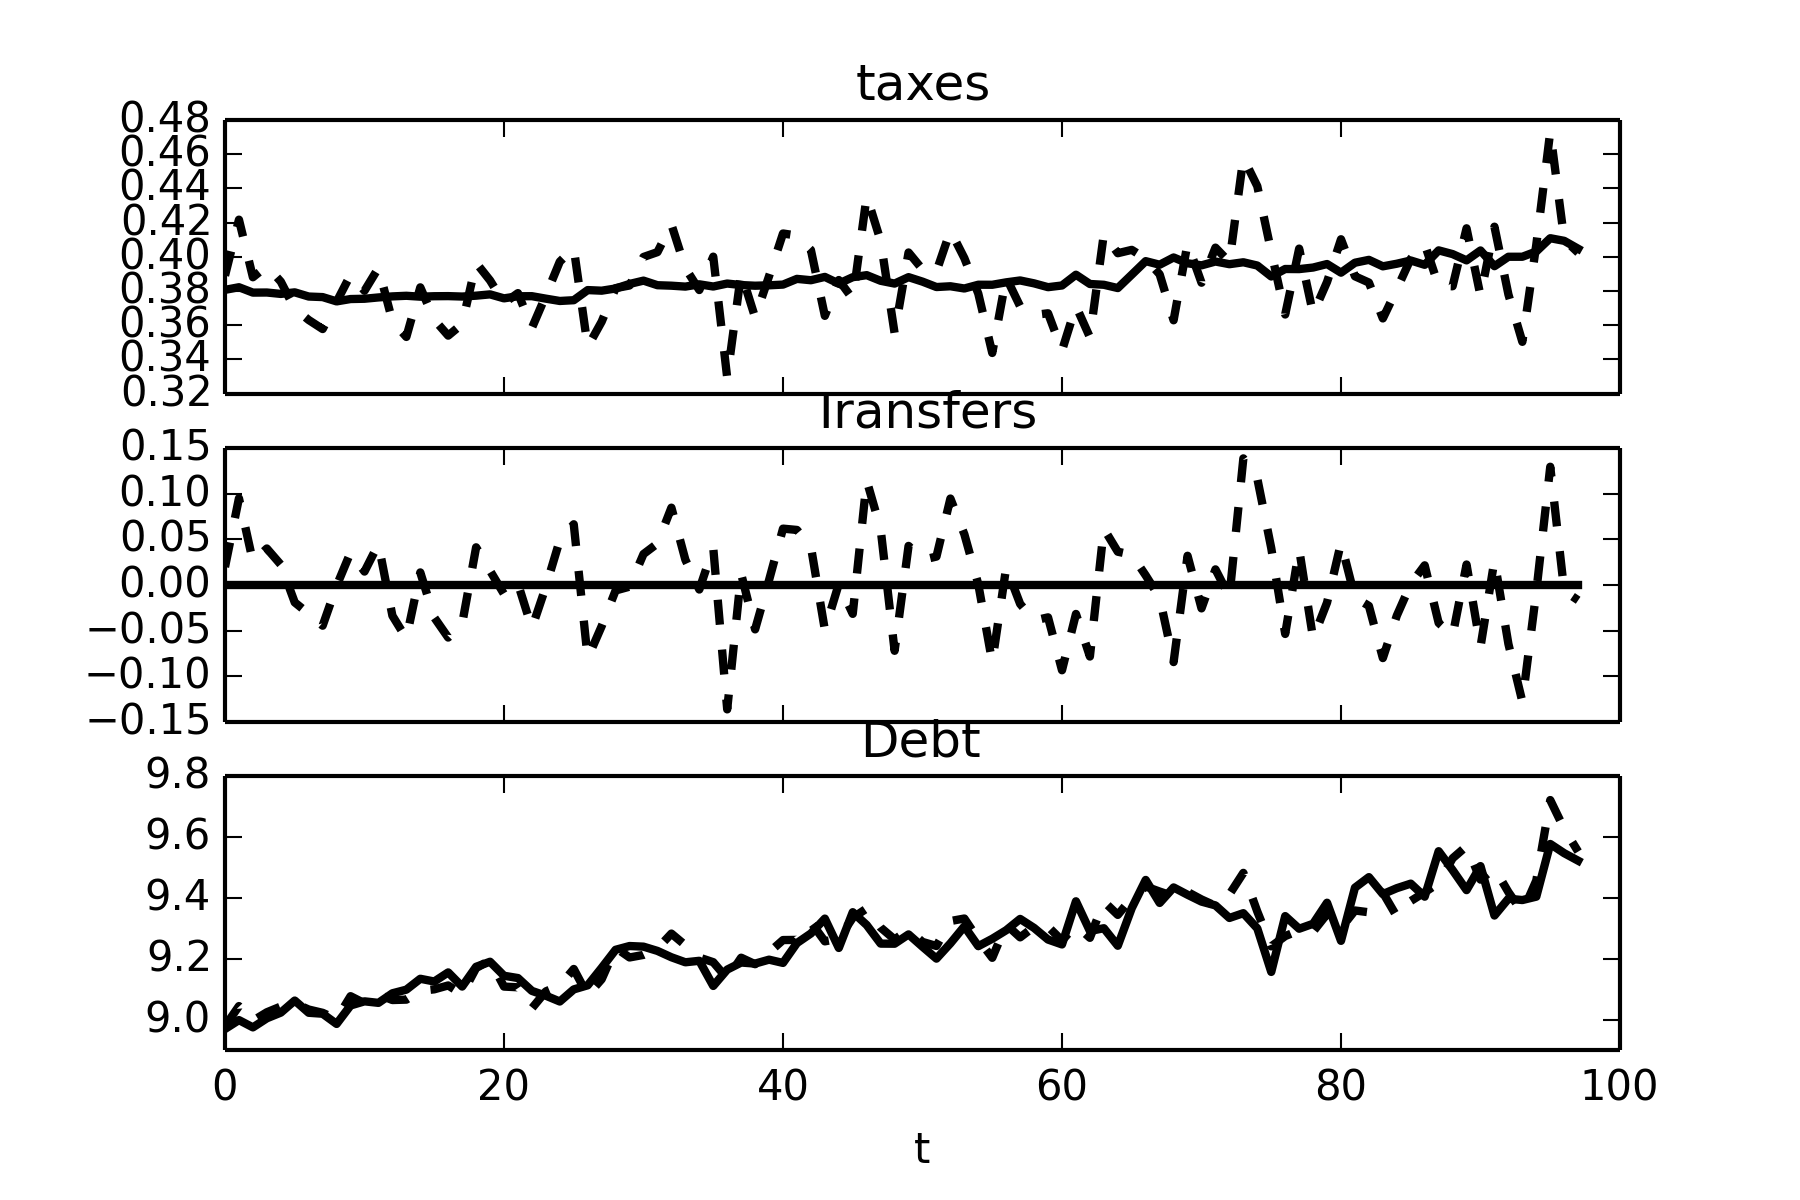
\includegraphics[width=\textwidth]{policy_long_sample_bond_economy.png}
\caption{\textbf{Bond Economy:}This plots a simulation for taxes, transfers and debt for 100yrs. The dotted line is the economy with i.i.d aggregate shocks}
\label{fig:}
\end{figure}


\begin{figure}[htp]
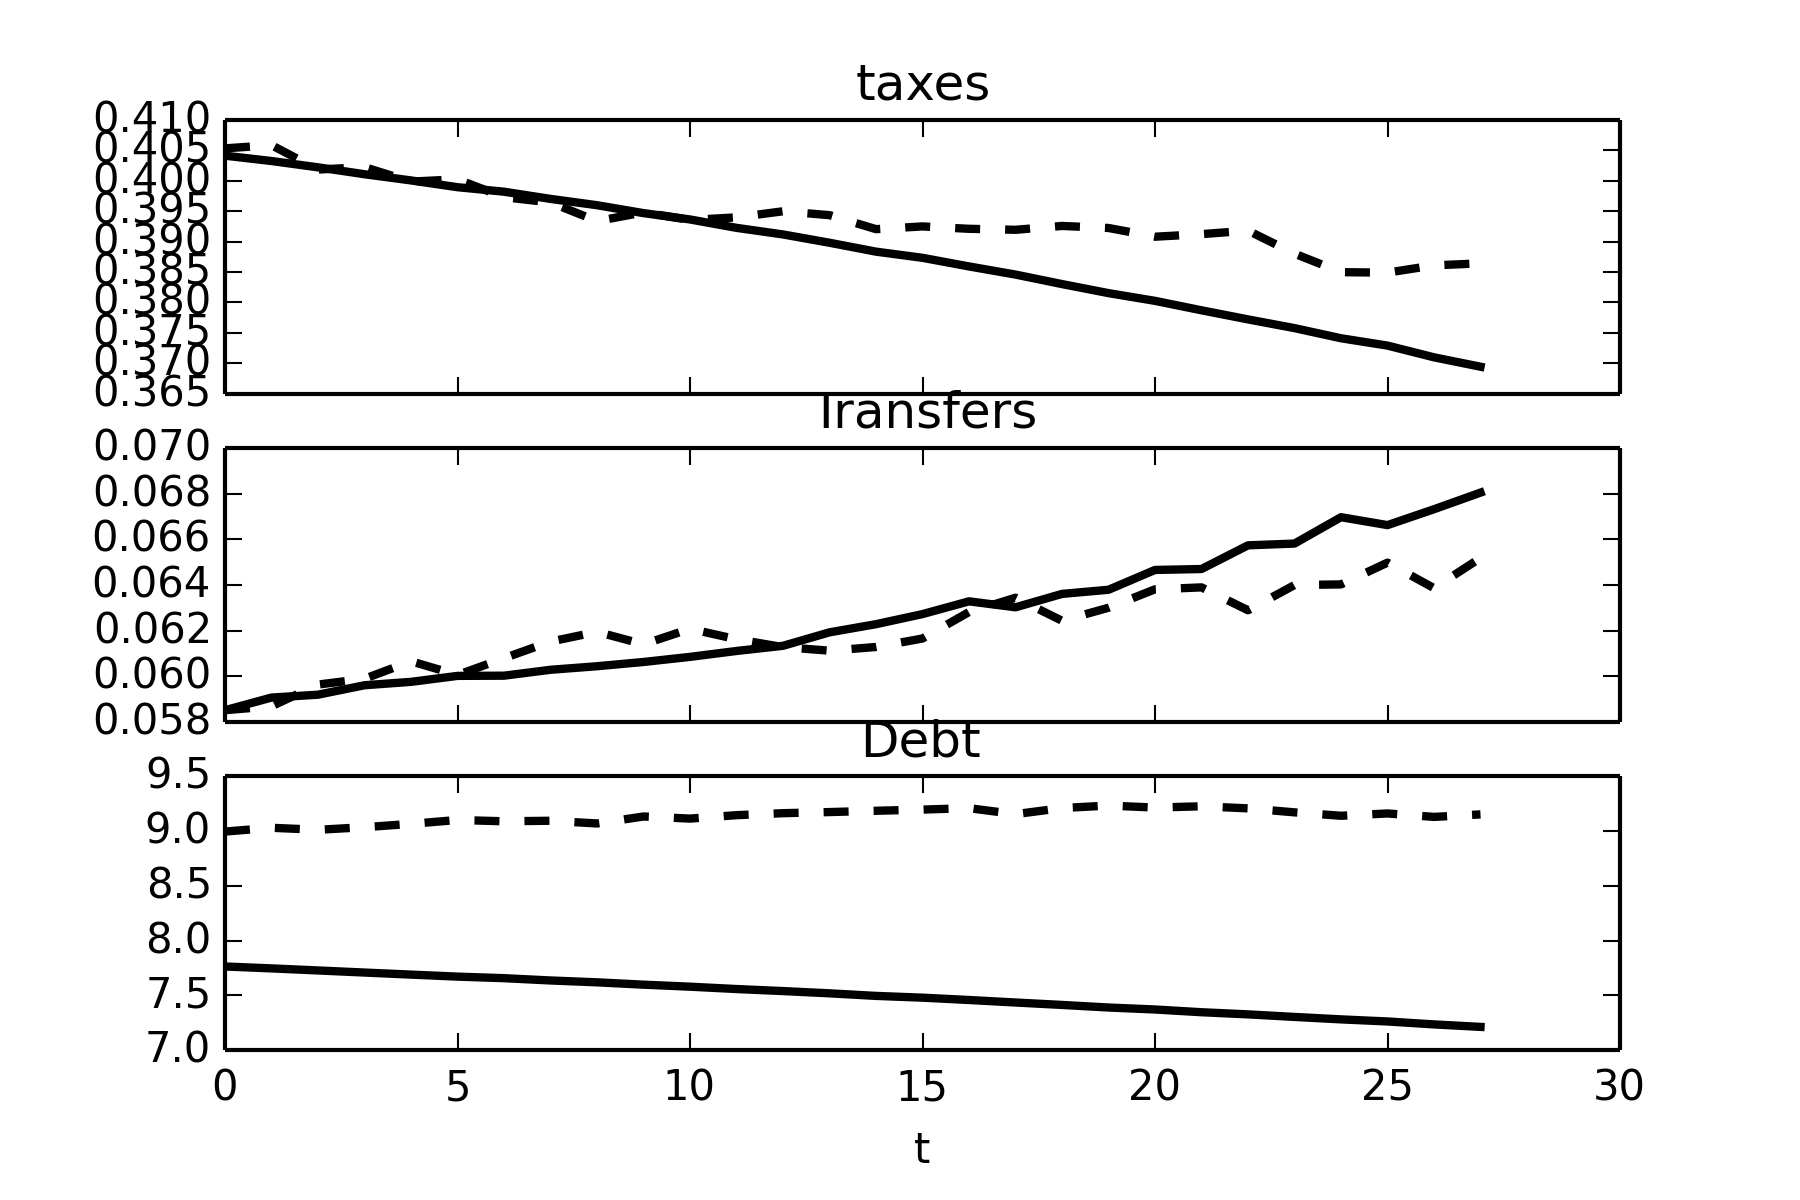
\includegraphics[width=\textwidth]{policy_drfits_bond_economy.png}
\caption{\textbf{Bond Economy:}This plots a simulation for taxes, transfers and debt for a sequence of high tfp (one std. deviation) shocks. The dotted line is the economy with idiosyncractic risk}
\label{fig:}
\end{figure}



\begin{figure}[htp]
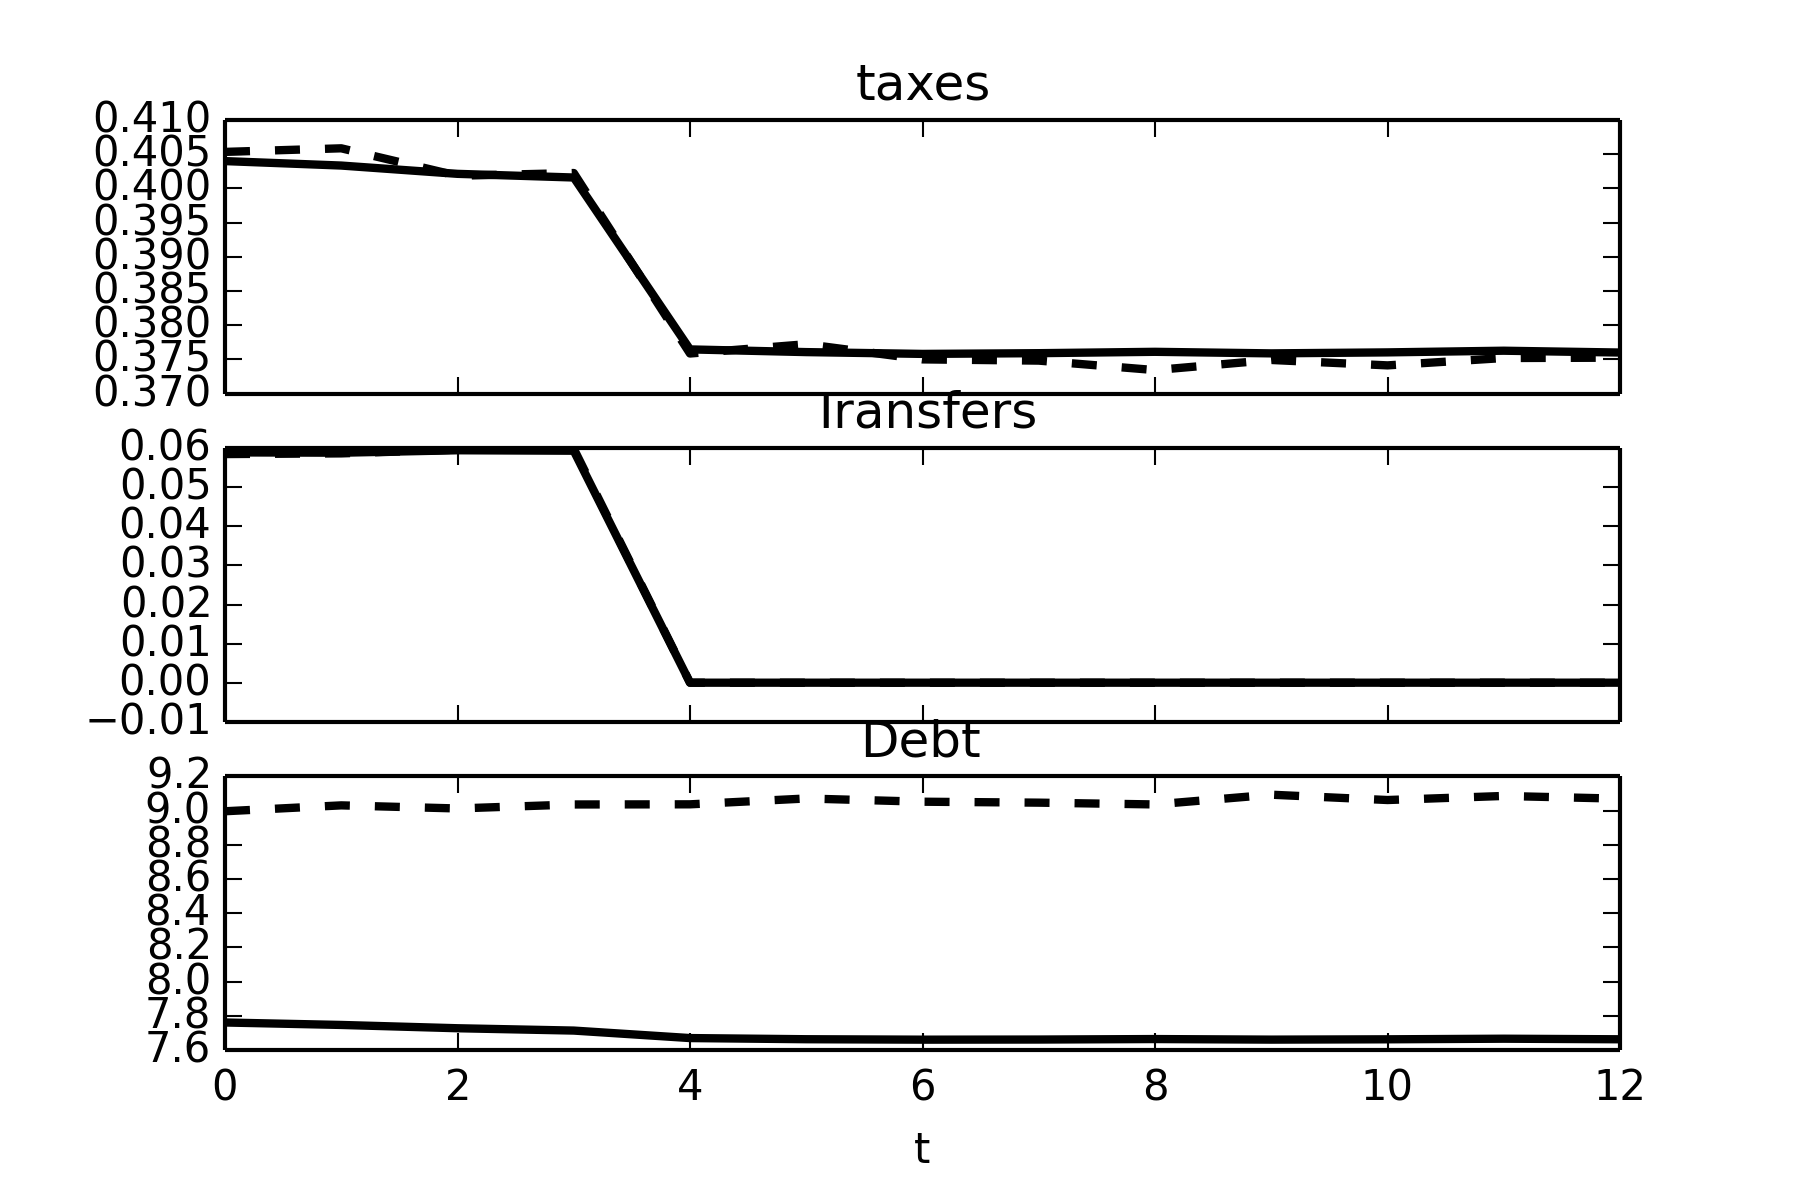
\includegraphics[width=\textwidth]{policy_irf_high_bond_economy.png}
\caption{\textbf{Bond Economy:} This plots a ``impulse response'' (5 period of high aggregate TFP followed by no aggregate shocks) for taxes, transfers and debt. The dotted line is the economy with idiosyncractic risk}
\label{fig:}
\end{figure}


\subsubsection{Procyclical Payoffs}

\begin{figure}[htp]
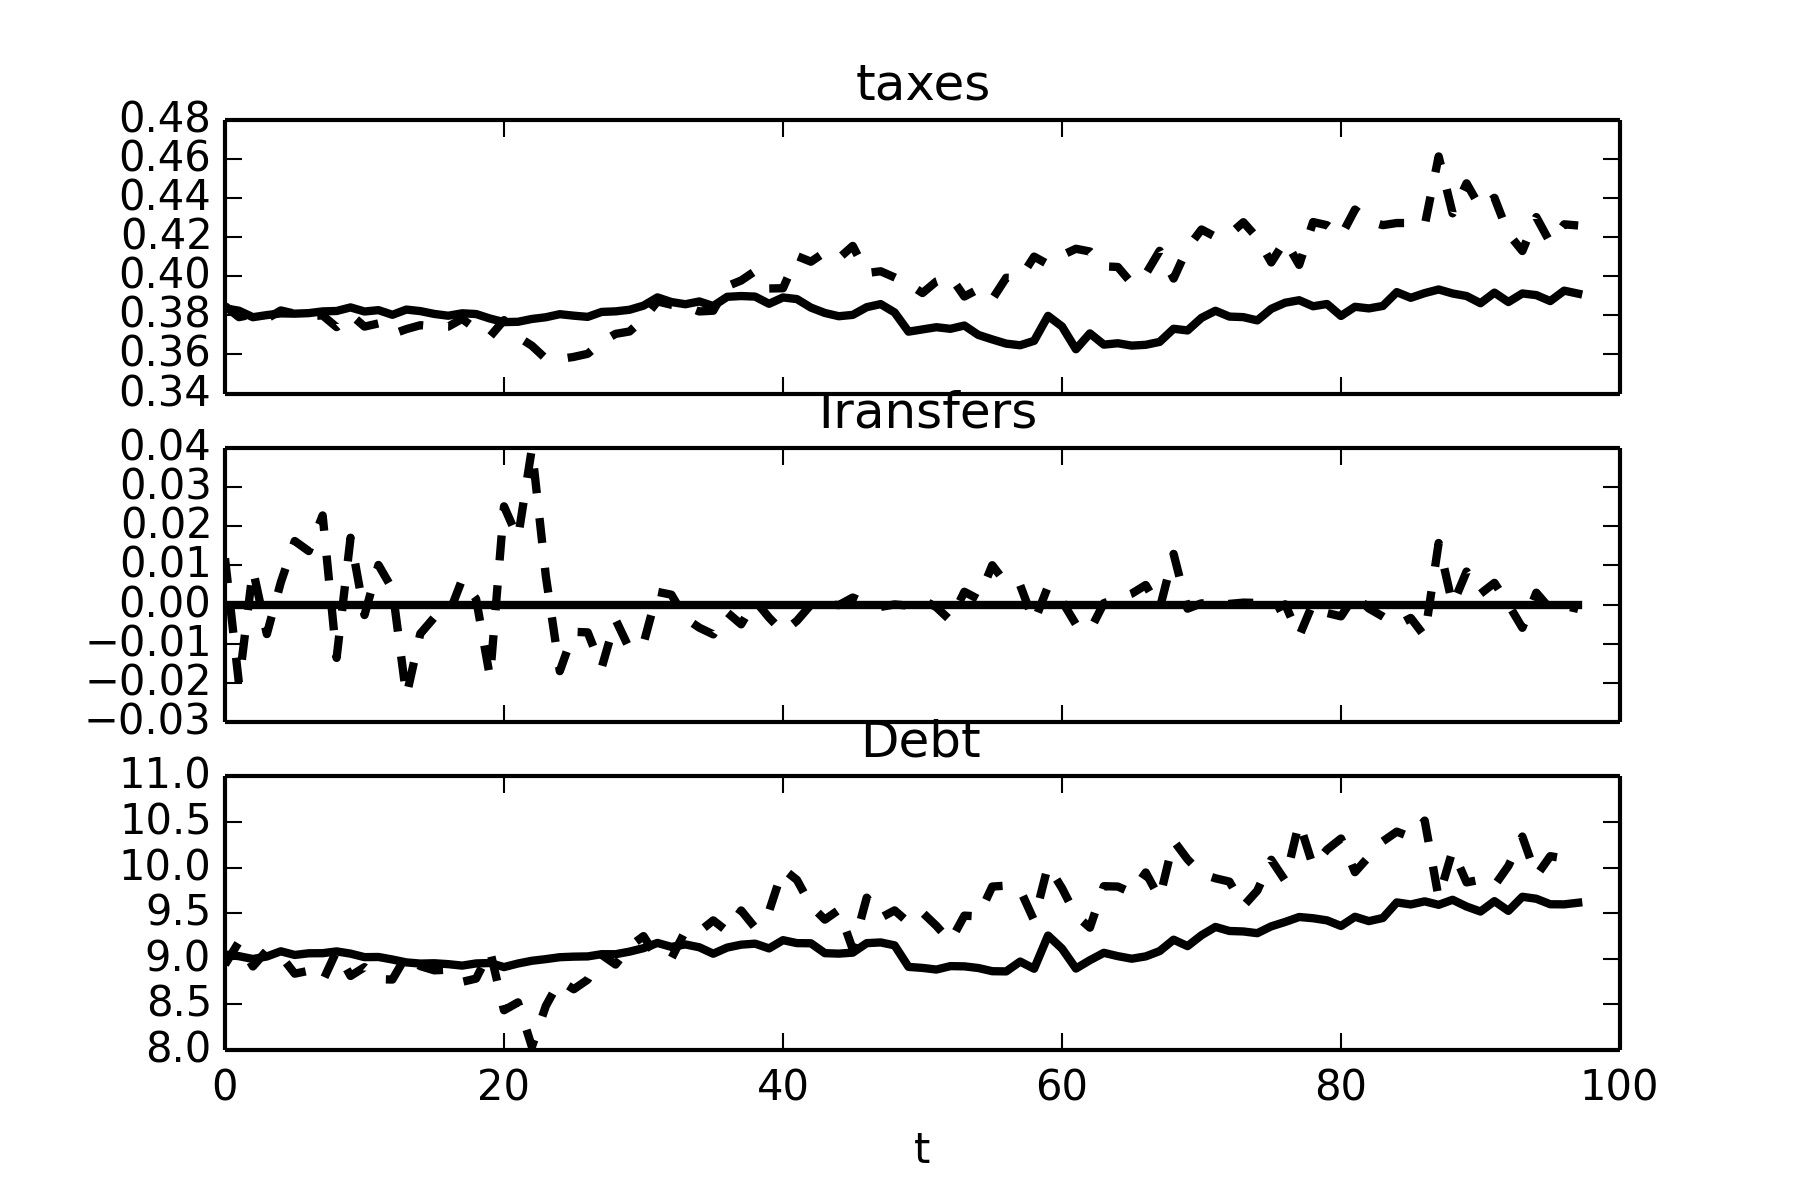
\includegraphics[width=\textwidth]{policy_long_sample_procyclical.png}
\caption{\textbf{Procyclical payoffs:} This plots a simulation for taxes, transfers and debt for 100yrs. The dotted line is the economy with i.i.d aggregate shocks}
\label{fig:}
\end{figure}


\begin{figure}[htp]
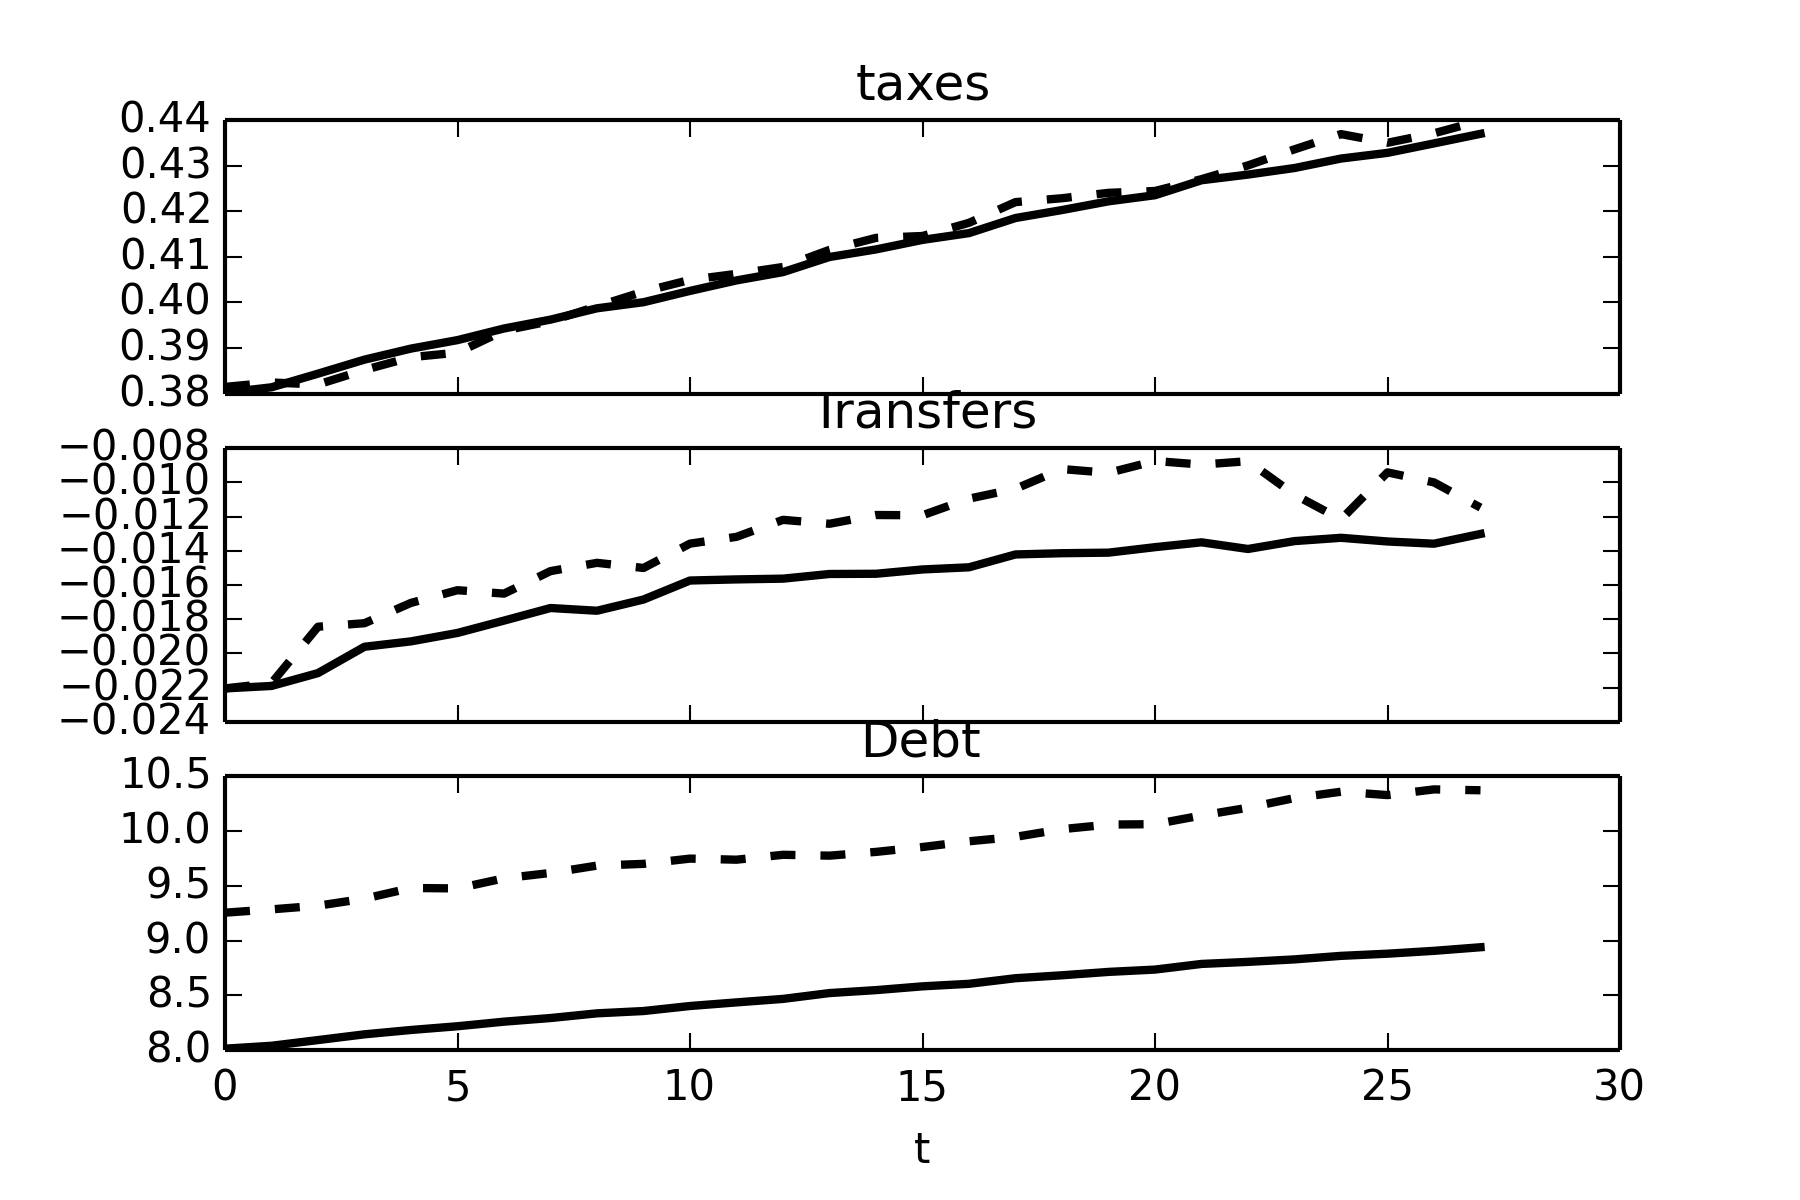
\includegraphics[width=\textwidth]{policy_drfits_procyclical.png}
\caption{\textbf{Procyclical payoffs:} This plots a simulation for taxes, transfers and debt for a sequence of high tfp (one std. deviation) shocks. The dotted line is the economy with idiosyncractic risk}
\label{fig:}
\end{figure}



\begin{figure}[htp]
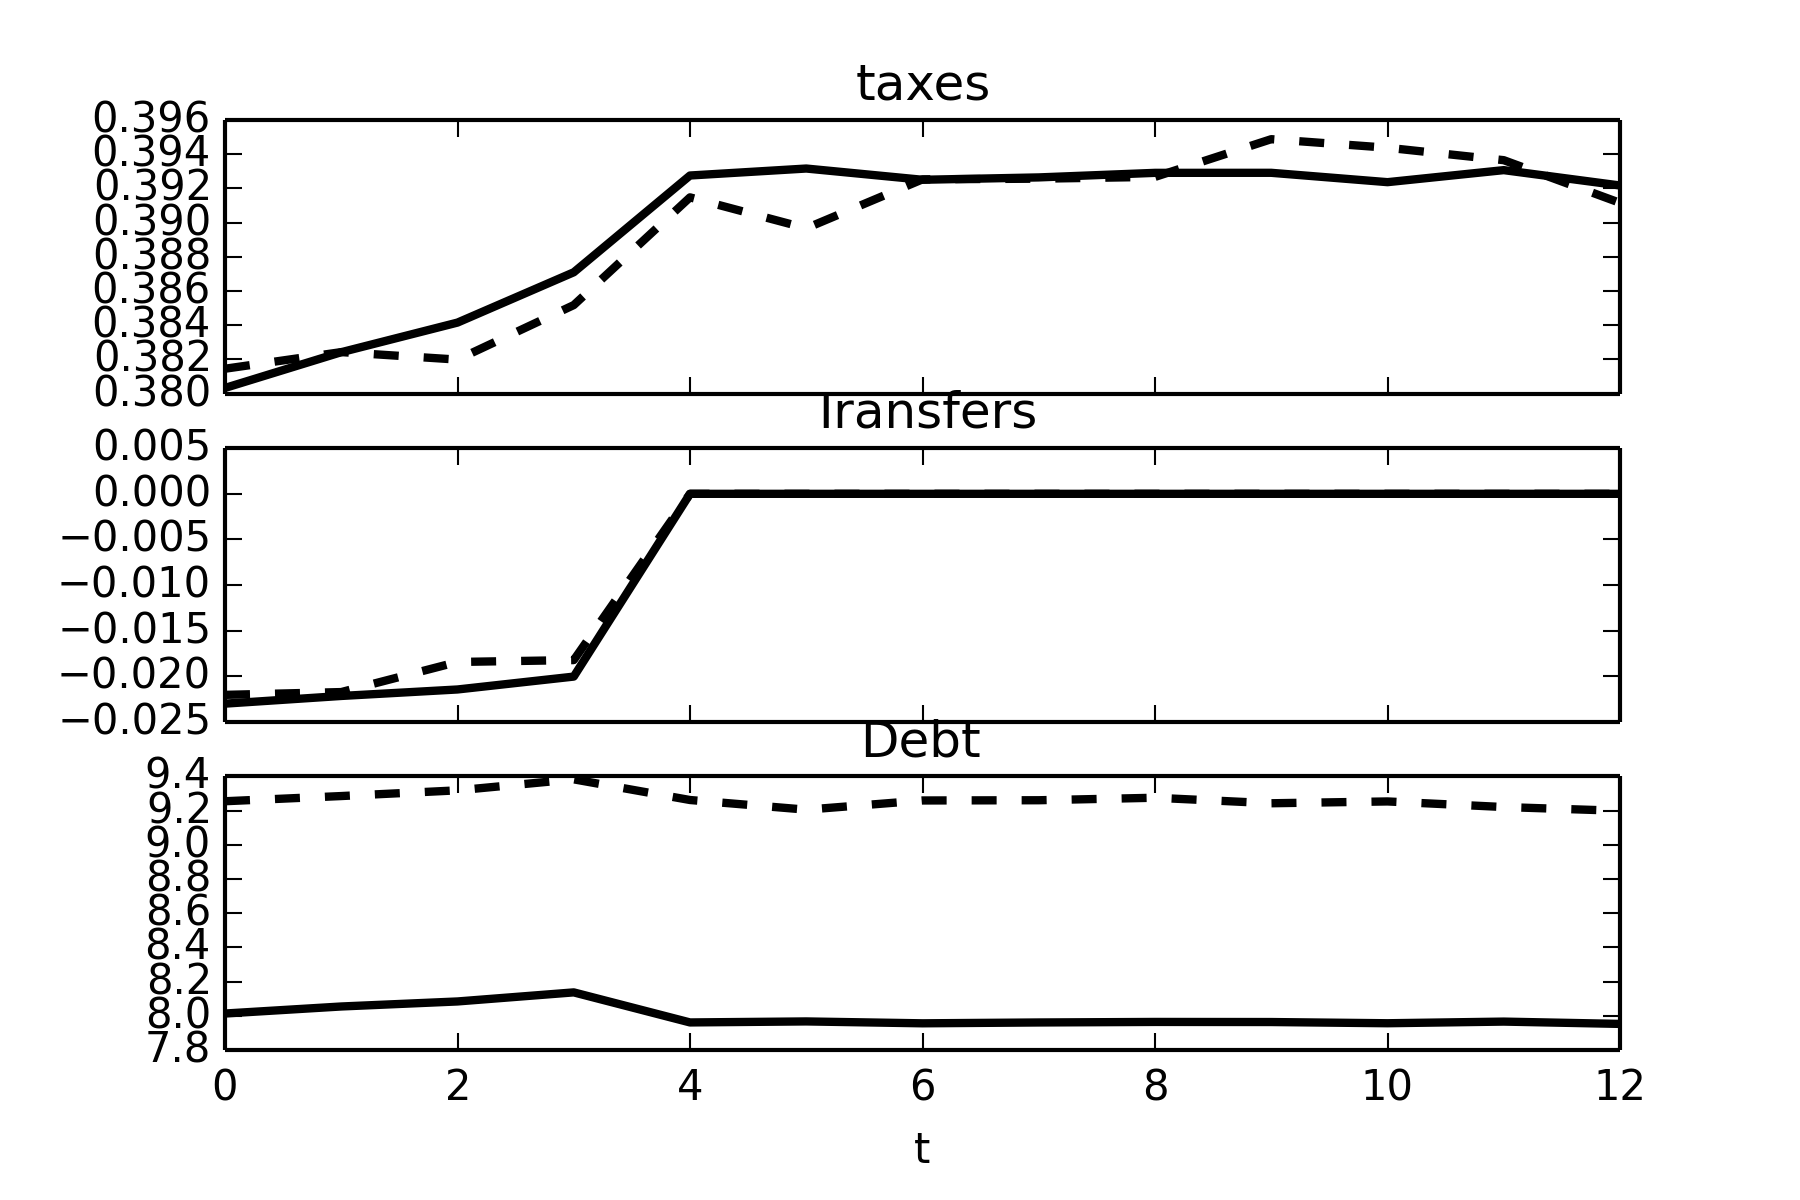
\includegraphics[width=\textwidth]{policy_irf_high_procyclical.png}
\caption{\textbf{Procyclical payoffs:} This plots a ``impulse response'' (5 period of high aggregate TFP followed by no aggregate shocks) for taxes, transfers and debt. The dotted line is the economy with idiosyncractic risk}
\label{fig:}
\end{figure}


\end{document}


\end{document}

\section{Some thoughts:}
\begin{itemize}

\color{red}{
\item We ran into problems here before discussing aggregate debt.  I think it would be best to talk about the distribution of debt, because of the Ricardian equivalence result.
\item  As I see it there are really too possibilities when we do the numerical exercise.  My prediction is that tax rate will have a high base level and the aggregate shocks will induce variation around that level.  If that is the case, I'm not sure how the discussion of payoffs adds to the paper.  We use it to discuss why the support of the distribution of taxes would be large, but if in the end the support of the distribution of taxes is tight it seems like we would only be confusing matters.
\item  I this case, I would just use the quasilinear example with two agents to demonstrate how transfers are distortionary.
\item  On the other hand if including aggregate shocks causes the tax rate to walk around a lot our results on the support of the distribution of taxes would fit in well with the paper.
}



\end{document}

\section{old notes}
\subsection{Quasi Linear with one productive agent}
We thought through the simple case you posed yesterday to contrast the effects of endogenous transfers. Here are the key outcomes. I might be repeating a few things we already discussed.

1] Representative agent economies with non-negativity constraints on transfers generically have zero distortionary taxes and FB level of assets for the government in the limit. 

2] We then looked at the economy with two agents who are quasilinear in consumption and one of the guys cannot work. There are no restrictions on transfers. Here are the outcomes and comments as we approach the limit of this economy when the unproductive agent has zero pareto weight. 

a) If there are no non-negativity constraints on consumption of the unproductive agent,  the Planner wants to drive his consumption to minus infinity (through lumpsum taxes) and  give labor  subsidy to finance the consumption of the productive agent.

b) Suppose we impose a non-negativity constraint on the consumption of the productive agent. The statement we have is

" There exists an threshold for the pareto weight of the productive agent such for an higher pareto weight, the allocation has two features
i) consumption of the unproductive agent is zero for all histories
ii) Labor taxes approach minus infinity and assets of the government reach infinity. 
 
Although distortionary taxes diverge, labor is bounded due to income effect. This keep the costs for the planner bounded.

Note that this solution does not violate no ponzi conditions as the debt accumulation is "slow". This is driven by the martingale component. Also consumption is bounded along the path. 

There is a threshold mass of unproductive agents such that below it, the limiting assets will be bounded and the planner would use both transfers and a positive subsidy. This comes from the fact that the costs of subsidies is bounded and costs of transfers are proportional to the mass of unproductive agents.

The  argument has two parts -  With risk free bonds the multiplier on the implementability constraint is a martingale that is bounded above by a positive constant. This bound comes from driving the implied taxes to minus infinity.
Next we show that if the value function is concave (we havent proved it yet..but it should follow from arguements that you had in your notes) the multiplier cannot converge to any other constant.

Our guess is that this is being driven by two forces - one active in AMSS and the other that comes from redistribution. The non-negativity constraint on consumption of agent two is effectively a non-negativity constraint on transfers. But  the government in our economy does not want to use transfers at the FB because it has to throw stuff in the ocean as it gives resources to an agent it does not care for. This extra consideration makes it accumulate even further assets and approach the limits we discussed in the statement before.



As compared to the representative agent model studied in BEGS2,we believe that there exists a lower bound on alpha ( being the pareto weight of the productive agent) such that for all alpha above this bound the optimal Ramsey allocations of the two agent economy matches that of the representative agent without lump sum transfers.  This includes all statements about restrictions on payoff vectors such that the invariant distribution is a single point. If the payoff vector is perfectly correlated with $g$ then for alpha above some lower bound the ergodic distribution is single point. Technically the 2 agent economy kills the first best as the absorbing state that arises in standard representative agent models with transfers. 

For alpha below this threshold there is a range of initial assets for which the  allocation is immediately in ``steady state'', in line with the theorem we had in the BEGS1.  In these steady states the non-negativity constraint on consumption will always be slack.  This range of steady states assets may depend on the payoff vector.  Furthermore, when the payoff vector is perfectly correlated with $g$ there should be an additional steady state analogous to those we studied in BEGS2, where the non-negativity constraint on consumption is always-binding.  As alpha approaches zero, the range of steady states such that the non-negativity constraint is slack approaches all feasible initial debt levels.






\subsection{Risk Aversion}


Consider a representative agent economy with incomplete markets where 
\begin{itemize}
\item The government trades an asset with payoff $\mathbf{p}=p(s)$
\item The agent values consumption and leisure with CES prefernces: $\frac{c^{1-\sigma}}{1-\sigma}-\frac{l^{1+\gamma}}{1+\gamma}$
\item The economy is subject to i.i.d expenditure shocks $g(s)$
\item For now, let us assume the government has no access to transfers
\end{itemize}

We are interested in characterizing the properties of the ergodic distribution of government debt $\lim_t b_t$ as we vary economies in $\mathbf{p}$ and $\sigma$.

Our plan is work on the following set of conjectures (given what we know in the economy with $\sigma=0$.)

\begin{enumerate}
\item There exists a subspace $\mathcal{P}=\{\mathbf{p}: \quad s.t \quad  \lim_{t}u_{c,t}b_t \text{ is degenerate }\}$ for a restricted set of initial $b_0$. It also implies that the debt $b_t$ will have a $S$ point discrete ergodic distribution. 

The qualification for the initial debt comes from our numerical work for two shocks iid case. We saw there that for a given payoff vector $\mathbf{p}$ there can exist more than one LS allocations indexed by respective initial debts that can be supported with  $\mathbf{p}$. 

. We might try to get a clean statement for the two shock bond economy where it looks like there is a unique steady state. 

\emph{With QL preferences we had a tighter characterization for $\mathcal{P}$. It was a subspace of the linear space spanned by $g(s)$. Furthermore the convergence to a degenerate level of debt was for all initial conditions}

\item In terms of the qualitative properties, we should be able to say something about sign and the magnitude of the steady state assets in terms of the strength of the covariance between marginal utility adjusted payoffs, $p(s)u_c(s)$ and marginal utility adjusted government surplus. 

\emph{This is very similiar to our result in QL economy, except that we could give a characterization interms of primitives $p(s)$ and $g(s)$}

\item We are trying to see if there is a systematic relationship between risk aversion ergodic debt. Numerically it looks like there is a postive relationship between $\sigma$ and the steady state (marginal utility adjusted) debt but it depends on the payoff vector. Things look wierd for very extreme payoffs. Maybe we can say something in the neighbourhood of a bond economy $\mathbf{p}\approx1$ or the risk neutral economy $\sigma \approx 0$ by extending the linearization techniques.


\end{enumerate}


